%!TEX root = ../dissertation.tex
%\begin{savequote}[75mm]
%Nulla facilisi. In vel sem. Morbi id urna in diam dignissim feugiat. Proin molestie tortor eu velit. Aliquam erat volutpat. Nullam ultrices, diam tempus vulputate egestas, eros pede varius leo.
%\qauthor{Quoteauthor Lastname}
%\end{savequote}

\chapter{Holographic approach to arbitrary-potential generation}

\section{Why do we need custom optical potentials?}
One of the advantages of cold-atom experiments is the ability to prepare and probe the system on its characteristic time and length scales (for lattice models, those would be a tunneling time and lattice spacing respectively). Quantum gas microscopy enables us to observe our lattice system with single site resolution, which led to the first single-site-resolved observations of superfluid to Mott insulator \cite{Bakr2010, Sherson2010} as well as paramagnet-to-antiferromagnet \cite{Simon2011, Mazurenko2017} quantum phase transitions. However, in order to fully enable the capabilities of such experiments, one needs a tool to arbitrarily control the shape of optical potentials in the system. Implementation of such techniques enabled the preparation of a variety of different initial states with high fidelity \cite{Preiss2015}, and studies of systems with complex \cite{Husmann2015, Valtolina2015} as well as dynamically changing \cite{Boyer2006} geometries. To achieve this, one has to control the light intensity on a single lattice site scale, which can be achieved by means of spatial light modulators (SLM).

\section{Spatial light modulators}
There are two main types of SLMs that are being used in such setups: liquid-crystal displays (LCD) and digital micro-mirror device (DMD). LCDs can be configured to provide amplitude modulation or phase modulation of the incident beam, using the birefringence of liquid crystals. With optimization and feedback algorithms \cite{Gaunt2012, Nogrette2014}, it is possible to create complex, re-programmable potentials, using this technology. However, this type of SLM has one major drawback when it comes to cold-atom experiments. Due to the nature of liquid crystals, they have to be placed into a switching electric field that oscillates with frequencies in the $kHz$ range, causing the output light to blink at the same frequency. This blinking could potentially be a problem since the typical trap frequencies of the atoms in optical lattice experiments lie in the same frequency range, and hence the blinking light might induce undesired heating in the system.

Another approach is to use a DMD, which consists of CMOS arrays of micromirrors on torsion hinges which can be switched
between two angles corresponding to the \textit{on} and \textit{off} directions. These devices are typically used in commercial video projectors and are available with resolutions up to $2560 \times 1600$ pixels. DMDs can statically hold a desired pattern for an extended period of time, which mitigates the blinking issue of LCDs. However, this comes at a cost since, in order to control the phase information of the outgoing wavefront, one has to use special techniques\cite{Lee1970, Goorden2014} that result in low power efficiency. 

The device used in our experiment is the Keynote Photonics FlexLight X3, which uses the Texas Instruments DLP 5500 chipset. The $1024 \times 768$ micromirror array has a pitch of $10.8 \mathrm{\mu m}$, micromirror tilts at $\pm 12^{\circ}$ from the normal, and an update rate of $5 \mathrm{kHz}$. The time required to switch between individual patterns is even shorter, on the order of a few $\mathrm{\mu s}$, which can allow dynamical control over the potential.

A straightforward way to use SLM in the microscope setup is by directly imaging it onto the atoms \cite{MaThesis, MarurenkoThesis}. The gray scaling of the image can be achieved by setting the magnification such, that a single lattice site corresponds to an area of the SLM that contains multiple pixels. This method is very powerful for creating large-scale, smoothly-varying potentials. However, there are two major challenges, that can limit the performance of the SLM in a real setup: \textit{First}, the wavelength of conservative light potentials, that one wants to project, is generally very different from the atom imaging wavelength, which most quantum gas microscopes are optimized for. This can lead to significant distortion of the desired wavefront due to chromatic aberrations if the imaging system is not specifically corrected for that. The first two leading orders of aberrations, in this case, are given by defocus and spherical aberration. This problem can be solved by either using an achromatic imaging system, that is wavelength insensitive in the desired range, or precompensating the imaged wavefront for the defocus caused by the imaging. \textit{Second}, it is fundamentally impossible to create $100 \%$ intensity modulation of the potential on the single site scale with the uniform phase of the electric field. 

\section{Enhancing the resolution through controlling the phase of the field}
To illustrate the last point, let's consider a single lens with a focal length $f$ and a fixed aperture of size $d$ in the Fourier plane (see fig~\ref{fig:DMD_lens}). To keep the math simple let's consider only two spatial dimensions $x$ and $z$. The sharpest single feature that one can make in the image plane with constant phase wavefront in the Fourier plane is the so-called point spread function, with the resulting light intensity in the image plane given by $I(x) \sim sinc^2(\frac{\pi}{\Theta} x)$, where $\Theta = \frac{\lambda f}{d}$ (see fig~\ref{fig:DMD_lens} A). The question becomes: how can one make an intensity pattern that is periodic with period $\Theta$? Two different electric field profiles would give us the intensity profile that satisfies this requirement: $E_1 \sim \sqrt{(1+cos(\frac{\pi}{\Theta}x))/2}$ and $E_2 \sim cos(\frac{\pi}{2\Theta} x)$, both yielding $I \sim (1+cos(\frac{\pi}{\Theta}x))/2$ (see fig~\ref{fig:DMD_lens} B,C). The first one has only positive electric field components and hence a uniform phase, however it's Fourier transform requires the Fourier plane, that is double the size of our initial point spread function. The second one has the same Fourier plane size as the one we started with at the expense of having electric field oscillate between positive and negative values, or in other words the phase of adjacent maxima alternate between $0$ and $\pi$. This example shows us, that using the phase control of the potential in the image plane, allows us to increase the image plane resolution by a factor of two for a fixed aperture in the Fourier plane.
%The characteristic size of the feature is $FWHM = 0.84 \Theta$.

\begin{figure*}[t]
	\centering
	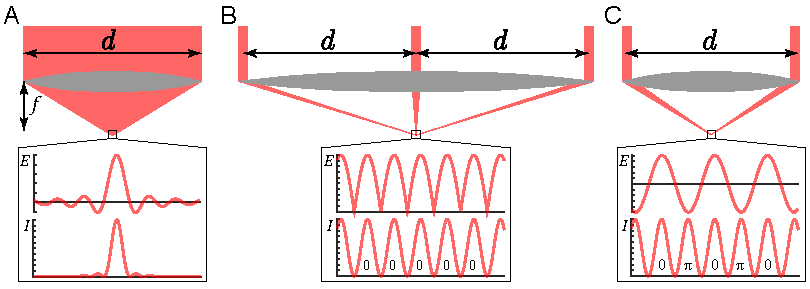
\includegraphics[scale=1]{figures/DMD_lens.pdf}
	\caption{{\bf Enhancing image plane resolution with phase control}. {\bf A} Homogeneous illumination of a lens with focal distance $f$ and a Fourier plane size $d$ results in so-called point spread function. It determines the size of the smallest point source feature, that can be resolved through such an imaging system. The zoom in shows the image plane electric field and intensity profile for each case. {\bf B} Double the size of the Fourier plane is required in order to make a periodic structure with, a period corresponding to the size of the point spread function from A, with a constant phase in the image plane. {\bf C} The pattern with the same periodicity can be created using the Fourier plane of the original size, however, the phase of the adjacent intensity maxima alternate between $0$ and $\pi$ in this case.}
	\label{fig:DMD_lens}
\end{figure*}

\section{Encoding phase information with a Fourier plane DMD}
Another practical challenge comes from the fact that every physical imaging system has aberrations. Hence, one needs to correct for all distortions that the beam encounters on its way from the DMD to the desired image plane (in our case, we call it the atom plane). Note, that one needs to correct for both the intensity pattern that illuminates the DMD as well as any phase deviation from the desired wavefront. The latter is particularly challenging for imaging systems with high numerical aperture, due to the breakdown of the paraxial approximation. In order to achieve the best possible quality of the optical potentials, it would be desirable to be able to measure and actively compensate for aberrations in the system. Here the use of the DMD in the Fourier plane becomes particularly useful.

\begin{figure*}[t]
	\centering
	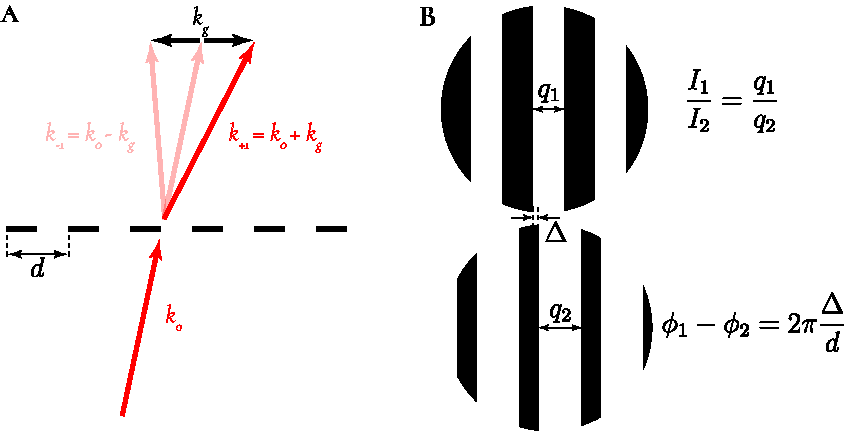
\includegraphics[scale=1]{figures/DMD_grating.pdf}
	\caption{{\bf Encoding phase and amplitude information with a grating}. {\bf (A)} When a light with initial wave vector $k_0$ passes through an amplitude grating with period $d$, its outgoing wave vector can be changed by any integer multiple of grating wave vector $k_g\propto \frac{1}{d}$. {\bf (B)} Two patches ($1$ - top, $2$-bottom) with the grating of the same period $d$ but different duty cycles $q_1$ and $q_2$ are shown. Since the duty cycle determines how much light passes through, the intensity $I$ of the outgoing light in each case is proportional to the duty cycle $\frac{q}{d}$. The information about the local phase of the grating is imprinted onto the phase of the outgoing electric field $\phi$.}
	\label{fig:DMD_grating}
\end{figure*}

the information about the local phase of the grating is imprinted onto th

Since DMDs don't have a built-in way to control the phase of the light field, one needs to find a way to encode this information using a binary structure of the DMD pixels. In our experiment we use a holographic approach that works as follows (see fig.~\ref{fig:DMD_grating}): Consider a plane wave incident onto an amplitude diffraction grating. The grating will create multiple diffraction orders on the output, each satisfying the condition $k_n = k_0 + n*k_g$, where $k_n$, $k_0$ and $k_g$ are the wave vector of the n-th diffraction order, the incident light and the grating, respectively. The grating wave vector is inversely proportional to the period of the grating $k_g \propto \frac{1}{d}$. We focus on the first diffraction order for the rest of the discussion. The overall spatial translation of the diffraction grating gets mapped onto the phase of the electric field in the diffracted order (see fig~\ref{fig:DMD_grating} B), whereas the ratio between the \textit{on} and \textit{off} pixels within one period of the grating (called the duty cycle) will result in the intensity modulation of the outgoing light. Therefore by controlling the phase and duty cycle of the underlying grating, we can locally control the phase and amplitude of the outgoing waveform at the DMD \cite{Zupanchich thesis}.

\section{Optical setup}
We chose to use an aperture of $500$ pixels (which approximately equals to $5.4 \mathrm{mm}$) in diameter on our DMD. In order to image it onto the objective Fourier plane, which is $18 \mathrm{mm}$ in diameter we use the optical set up shown in figure~\ref{fig:DMD_setup} A. In order to make the alignment easier and also to be able to control the image plane position of the potential without changing the hologram we use IP and FP mirrors (see fig.~\ref{fig:DMD_setup}). The FP mirror moves the beam primarily in the Fourier plane, since it's located very close to the intermediate image plane of the imaging system, and hence does not change the position of the beam in the image plane. The IP mirror position is chosen to be close to the Fourier plane, such that it primarily displaces the beam in the image plane. In order to understand the exact location of this mirror, it is instructive to look at where the plane of the DMD (which is the Fourier plane of the overall imaging system with respect to the atoms) is imaged to (see fig~\ref{fig:DMD_setup} B). It is clear from the figure that this mirror is positioned exactly in the Fourier plane of the imaging system and hence moves the beam in the image plane.

Typically, we use the DMD to create potentials that have single-site resolved features in one direction and a slowly varying amplitude in the other direction. The Fourier transform of such a pattern occupies the entire Fourier plane along the direction of the narrow feature and only a small fraction along the other one which is inversely proportional to the size of the slowly varying amplitude. This implies that, if we would like to achieve the best power efficiency, we would like to match this profile with the intensity of the incoming beam. We accomplish this with an additional elliptical illumination channel with aspect ratio $\frac{1}{7.5}$. The round illumination beam is primarily used for calibration purposes.

Since the DMD and the optical lattice don't have a common interferometric reference their relative position may drift in time. This means that we need a way to track and stabilize their relative alignment. We do so by imaging the reflections off the super-polished substrate of both the lattice and the DMD on a separate camera in the intermediate image plane (see fig.~\ref{fig:DMD_setup}). This method provides us with a reference that almost coincides with the atom plane. We apply feedback using the IP mirror of the DMD once every experimental cycle, corresponding to a frequency of $\sim 17 \mathrm{mHz}$. This allows us to stabilize the relative position to within $0.03$ lattice sites RMS. The residual noise is attributed to air currents and mechanical vibrations of the breadboards.

\section{Calibration and aberration correction}
In order to achieve a diffraction-limited resolution in the atom plane, we need a way to map out the aberrations that occur on the optical path from the DMD to the atom plane. The two main sources of the phase error in our system are the curvature of the DMD chip that is present due to the manufacturing process, and chromatic aberrations of the objective lens, which has a $\sim 1 \frac{\mathrm{\mu m}}{\mathrm{nm}} $ chromatic shift. We also need to compensate for the intensity profile of the beam that illuminates the DMD, in order to have spatial control over the amplitude of the electric field.

\begin{figure*}[t]
	\centering
	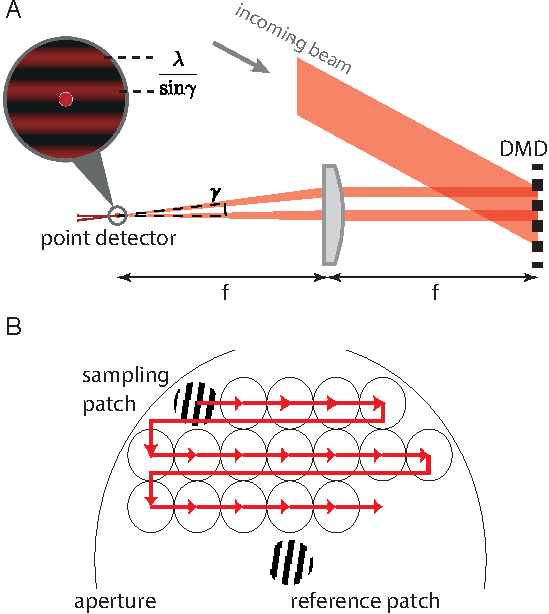
\includegraphics[scale=1]{figures/DMD_ipcal.pdf}
	\caption{{\bf Intermediate plane calibration}. {\bf (A)} The interference of two Fourier plane beams, created by small patches on the DMD, results in the sinusoidal intensity modulation in the image plane. The period of which is inversely proportional to the distance between the patches in the Fourier plane and the phase is equal to the phase difference between the two beams. The intensity profile is measured using point detector. {\bf (B)} During the calibration prcedure the reference patch remains static while the sampling patch scans across the entire aperture of the DMD. Figure adapted from \cite{Zupancic2016}.}
	\label{fig:DMD_cal_scheam}
\end{figure*}

An aberration-free lens bends a beam parallel to the optical axis such that it passes through the focal point, and makes the phase of any such beam equal at that spot. If we take two beams in the Fourier plane, they will interfere to create a periodic intensity modulation in the image plane, with a period inversely proportional to their spacing in the Fourier plane (see fig.~\ref{fig:DMD_cal_scheam}). The global phase of this modulation is given by the relative phase between the beams, and the amplitude is proportional to the product of electric fields. Hence, by using one beam as a reference one can map out the relative phase and amplitude of any other beam by measuring the phase and amplitude of the resulting interference pattern \cite{Zupancic2016}.

First, we perform the calibration in the intermediate image plane. A photodiode with a pinhole is used to detect the resulting intensity modulation (for a more detailed description of this procedure see the Master’s thesis by Philip Zupancic \cite{ZupancicThesis}). The size of the pinhole (in our case $10 \mathrm{\mu m}$) is chosen such that it is much smaller than the smallest period of the intensity modulation in the corresponding image plane, created by interfering two beams from the opposite ends of the Fourier plane. We use patches with diameter $\sim \frac{1}{15}$ of the full Fourier plane to create local beams from the previous example. This procedure is relatively fast and has a high signal to noise ratio, resulting in a typical wavefront flatness of $\sim \frac{\lambda}{40}$. By using a series of single reference patches we are also able to create an amplitude map of the illumination beam \cite{Zupancic2016}.  

\begin{figure*}[t]
	\centering
	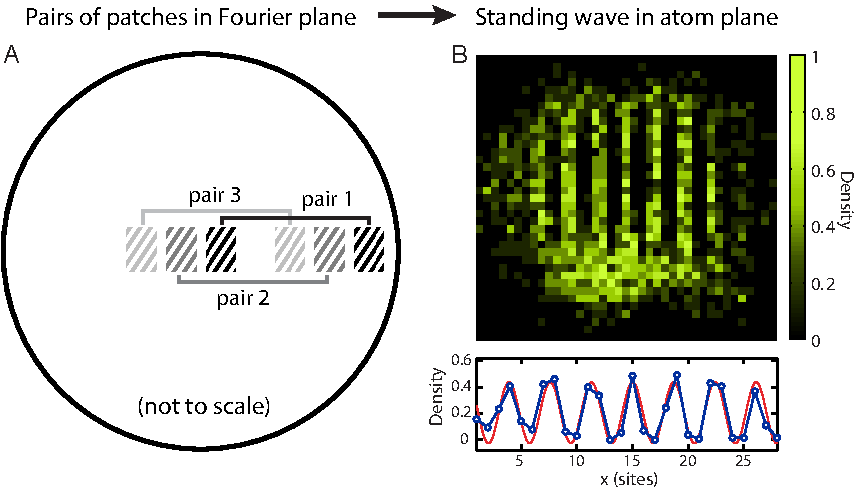
\includegraphics[scale=1]{figures/DMD_cal_atoms.pdf}
	\caption{{\bf Mapping out the phase with atoms}. {\bf (A)} A pair of patches with a fixed spacing results in the intensity modulation, which repel the atoms form the intensity maxima. In order to keep the pattern spacing fixed in the image plane the patches are translated together across the Fourier plane. {\bf (B)} An example $2D$ atom-density distribution (top) and average over the $y$ direction (bottom). The high contrast oscillations allow us to fit $\sim 7$ periods of modulation across the cloud.  Figure adapted from \cite{Zupancic2016}.}
	\label{fig:DMD_FPcal}
\end{figure*}

Next, we apply a similar technique to create a phase map from the intermediate plane to the atom plane, using atoms as a detector. We use weekly a weakly-interacting BEC of $\sim 400$ atoms in a harmonic trap with a diameter of $\sim 30$ lattice sites to read off the phase of the interference pattern. The intensity profile results in a density modulation of the atomic cloud due to the Stark shift exerted onto the atoms by the light (see fig.~\ref{fig:DMD_FPcal}). This technique has a number of limitations: since we rely on atoms to map out the resulting intensity pattern, we require at least a few oscillations of the potential within our cloud size. This limits our ability to measure a potential with large spacing or, from the Fourier plane perspective, patches that are close together. On the other hand, the patches at the opposite ends of the Fourier plane aperture, are also challenging to measure, since they result in an intensity modulation with a period of $\sim 1$ lattice site. Hence, using the same technique with a fixed reference patch that was used in the intermediate plane does not seem feasible. It is also challenging to acquire enough statistics in order to properly map out the intensity of the resulting potential, so the creation of the amplitude map is not feasible either. Here, one should note that the amplitude map should stay unchanged from the intermediate plane since there is no spatial dependence of the transmission of the optical elements in between the two planes. Hence, it is sufficient to use the amplitude calibration from the intermediate image plane all the way to the atom plane.

In order to overcome the above limitations, instead of keeping one patch as a reference we keep the spacing between two patches fixed and then scan this pair across the Fourier plane (see fig.~\ref{fig:DMD_FPcal}). The spacing is chosen such that the resulting intensity modulation has a period of $\sim 4$ lattice sites, allowing us to fit $\sim 7$ periods of modulation across the cloud. The resulting atom density distribution is averaged over multiple experimental realizations for a given pair of patches. During this measurement, any relative drift between the DMD pattern and the lattice directly results in an error of the extracted phase. Therefore, we use our DMD tracking routine during the measurement to illuminate this source of error. We extract the phase difference between a pair of patches by fitting a sine-wave to the resulting average density distribution. This procedure leads to a $66\%$ confidence interval of the fit for the phase estimation of $0.27 \mathrm{rad}$ or $\sim \frac{\lambda}{23}$.

Since we only measure the difference between a pair of patches, we effectively measure the derivative of the phase profile with this method. We reconstruct the phase by using a polynomial fit up to $7\mathrm{th}$ order. This procedure gives us a phase profile of the wavefront along one line. In order to reconstruct the full $2\mathrm{D}$ map we repeat this process along 6 different cuts through the Fourier plane, and then use a smooth surface parametrized by the Zernike polynomials up to the $6\mathrm{th}$ order to fit the full $2\mathrm{D}$ surface. Since, in the typical experimental setting we only use a small part of the Fourier plane for our patterns, after applying the full $2\mathrm{D}$ phase correction according to the reconstructed phase front, we repeat the calibration along the line through the center of the pattern region. The above procedure results in the RMS error of the phase between two patches on opposite sides of the Fourier plane being better than $\frac{\lambda}{14}$.

\section{Holographic potentials and their limits}
To create a desired potential on the atoms we rely on the imaging system property that the electric field in the image plane is the Fourier transform of the field in the Fourier plane. Therefore, in order to create a desired potential, we first numerically find its Fourier transform (note that in general, it will be a complex-valued function). Then, in order to represent both amplitude and phase information of the desired potential we, use the grating method, which encodes them in the local phase and duty cycle of the grating respectively. As long as we know the aberration profile in our system, we can correct for it by locally modifying the phase to $\phi_{total} = \phi_{target} - \phi_{aberrations}$ and amplitude $A_{total} = \frac{A_{target}}{A_{beam}}$.

If our DMD had pixels with a gray scale, the potential would be limited by the discretization of individual pixels, however the binary nature of the device create additional noise that limits the precision of the resulting potentials. One straightforward way to binarize the hologram is to switch the pixel with index $(i,j)$ \textit{on} if 
\begin{equation}
\left| (k_x i + k_y j + \phi_{total}) \; mod \: 2 \pi \right| < arcsin(A_{total}),
\end{equation}
and \textit{off} otherwise. Here $k_x$ and $k_y$ are $x$ and $y$ components of an a priori chosen wave vector of the underlying grating. This method has one straightforward problem, namely when one of the components of the grating wave vector is zero. In this case the stripes of the grating exactly coincide with pixels of the hologram, and if the wave vector is not equal to an integer number of pixels, result in the distortion of the desired potential (see fig.~\ref{fig:DMD_K_rotation}A). This problem can be avoided by slightly randomizing the pixels at the edges of the grating slits, using the function 
\begin{equation}
\frac{1}{2}(tanh((p(i,j) + arcsin(A_{total}))/\xi) - tanh((p(i,j) - arcsin(A_{total}))/\xi)),
\end{equation}
where $p(i,j))=\left| k_x i + k_y j + \phi_{total} \; mod \: 2 \pi \right|$ and $\xi$ is a parameter that controls the "smoothness" of the distribution (see fig.~\ref{fig:DMD_K_rotation} A inset). Now we compare if the value of this function at any pixel position is greater than a randomly chosen number between $0$ and $1$, we set pixel \textit{on} and \textit{off} otherwise. 

To study the effects of the smoothing potential, we perform numerical studies of the holograms. We use a fast Fourier transform (FFT) to determine the resulting image plane potential corresponding to a given hologram. In this study, we always compare a binarized hologram to its gray-scale counterpart, such that the binarization noise due to the finite size of the physical pixels is identical for both. From figure~\ref{fig:DMD_K_rotation}A it is clear that this method helps to reduce the effect of "bad" grating alignments, however, it comes at the cost of increasing the overall noise of the potential. This is easy to understand, since the more random we make the potential, the more likely it is to flip an otherwise correct pixel value. It follows from the discussion above that, in order to achieve the best performance with the holograms, it is beneficial to use a nearly deterministic method of binarization away from "bad" angles. 

\begin{figure*}[t]
	\centering
	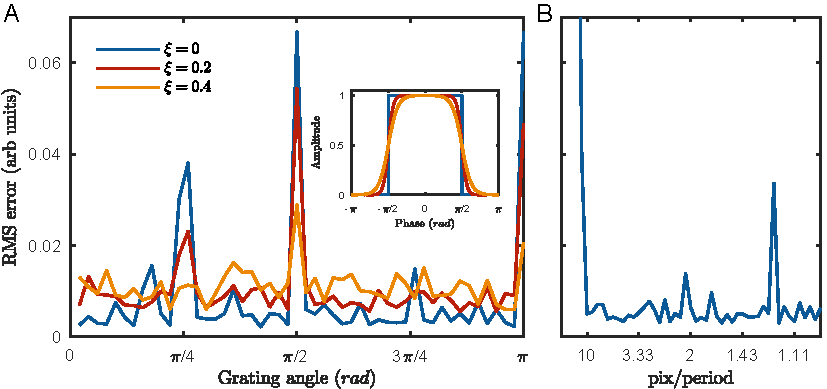
\includegraphics[scale=1]{figures/DMD_K_rotation_v3.pdf}
	\caption{{\bf Potential quality as a function of grating angle}. {\bf (A)} RMS difference of the image plane potential created by a binary hologram compared to the gray-scaled one, for different values of smoothing parameter. Pronounced peaks at $\pi$ and $\frac{\pi}{2}$ correspond to the situation when the grating aligns to the DMD pixels that leads to aliasing. Smaller peaks at $\frac{\pi}{4}$ and $\frac{3\pi}{4}$ correspond to the grating that runs diagonally to the pixels, which also suffer from the same problem. The imbalance between the minor peaks ($\frac{\pi}{4}$ and $\frac{3\pi}{4}$) is due to the test pattern shape, which is elongated along the $\sim \frac{\pi}{4}$ direction in the Fourier plane. Increasing the smoothening parameter decreases the sensitivity to the "bad" angles. However, it also decreases the overall quality of the resulting potential due to the inherent randomness of the method. The inset shows the smoothing function for the shown parameters. {\bf (B)} RMS difference of the image plane potential for deterministic binarization method ($\xi = 0$) as a function of grating period. Again for most of the values, the resulting pattern quality remains high. Interestingly the method works even when the period becomes smaller than $2$ pixels.}
	\label{fig:DMD_K_rotation}
\end{figure*}

\begin{figure*}[t]
	\centering
	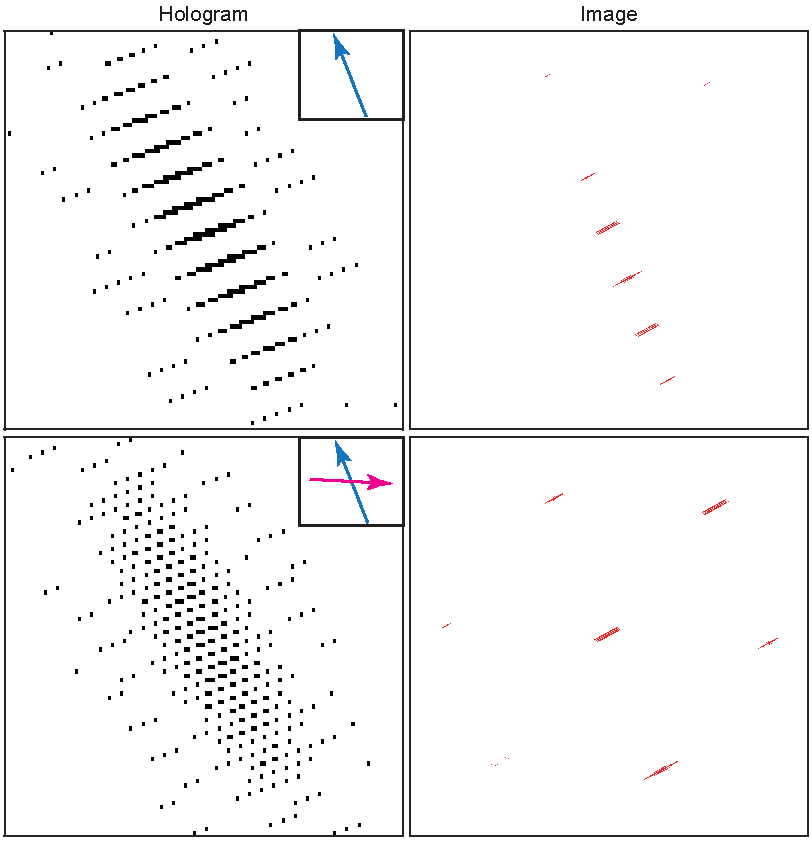
\includegraphics[scale=1]{figures/DMD_grating_bad_angle.pdf}
	\caption{{\bf Binarization artifacts}. On the right, examples of the binarized holograms for underlying grating period greater then two pixels (top) and lower then two pixels (bottom). The directions of the resulting wave vectors are shown in the inset.  On the left, the resulting intensity pattern in the image plane. Multiple images along the direction of the wave vector correspond to the different orders of the grating. For the case of smaller grating period, the binarized hologram develops a secondary wave vector, leading to the formation of multiple additional image plane fetchers.}
	\label{fig:DMD_grating_bad_angle}
\end{figure*}

Another parameter that could affect the hologram quality is the absolute value of the grating wave vector, or, in simple terms, the period of the stripes. Although one might expect to find some optimal value for this parameter, our numerical simulations show that the quality of the resulting potential stays unaffected in a wide range of parameters (see fig.~\ref{fig:DMD_K_rotation}B). Surprisingly, even when the stripe width becomes very small (less than $2$ pixels per period),  the image is not affected too much. In such a situation an additional grating emerges (see fig.~\ref{fig:DMD_grating_bad_angle}), resulting in additional images. However, those can be removed by spatial filtering.
 
We also try to determine the optimal value of the parameter $\xi$. To do that, we take the difference between two cuts that are separated by one lattice site through the resulting image plane profile. The introduction of the random parameter makes the resulting image plane profile vary slightly from realization to realization. Therefore, one can ask the question. What is the probability to obtain a pattern with the desired maximum difference between two cuts? Our numerical results suggest that the introduction of a small amount of randomness ($\xi \sim 0.04$) can increase the probability of obtaining a desired potential quality compared to the strictly deterministic case. Although more complex way to reduce the binarization artifacts like error diffusion algorithms \cite{floyd, Hu2018} have been studied, their application to our system does not improve the results. 

